\documentclass[a4paper,14pt]{article}
\usepackage[a4paper, mag=1000, left=2.5cm, right=1cm, top=2cm, bottom=2cm, headsep=0.7cm, footskip=1cm]{geometry}
\usepackage[utf8]{inputenc}
\usepackage[T2A]{fontenc}
\usepackage[english,russian]{babel}
\usepackage{indentfirst}
%\usepackage[dvipsnames]{xcolor}
\usepackage[colorlinks]{hyperref}
\usepackage{amsfonts} 
\usepackage{amsmath}
\usepackage{graphicx}
\usepackage{float}

\DeclareGraphicsExtensions{.png,.jpg}

\usepackage{fancyhdr}
\pagestyle{fancy}
\fancyhead[LE,RO]{\thepage}
\fancyfoot{}

\usepackage{listings}

\hypersetup{linkcolor=black}

\title{non-linear equations}
\author{Иван Золин}
\date{2023}
\thispagestyle{empty}
\begin{document}
	
	\begin{titlepage}
		\begin{center}
			\textsc{
				Санкт-Петербургский политехнический университет имени Петра Великого \\[5mm]
				Институт прикладной математики и механики\\[2mm]
				Высшая школа прикладной математики и физики            
			}   
			\vfill
			\textbf{\large
				Математическая статистика\\
				Отчёт по лабораторным работам №5-8 \\[3mm]
			}                
		\end{center}
		
		\vfill
		\hfill
		\begin{minipage}{0.5\textwidth}
			Выполнил: \\[2mm]   
			Студент: Золин Иван \\
			Группа: 5030102/00201\\
		\end{minipage}
		
		\hfill
		\begin{minipage}{0.5\textwidth}
			Принял: \\[2mm]
			к. ф.-м. н., доцент \\   
			Баженов Александр Николаевич
		\end{minipage}
		
		\vfill
		\begin{center}
			Санкт-Петербург \\2023 г.
		\end{center}
	\end{titlepage}
	
	\tableofcontents
	\newpage
	\listoffigures
	\newpage
	\listoftables
	\newpage
	
	\section{Постановка задачи}
	\textbf{Постановка задачи.}
	Исследование из области солнечной энергетики [1]. На рис 1 показана схема установки для исследования фотоэлектрических характеристик.
	\begin{figure}[H]
		\centering
		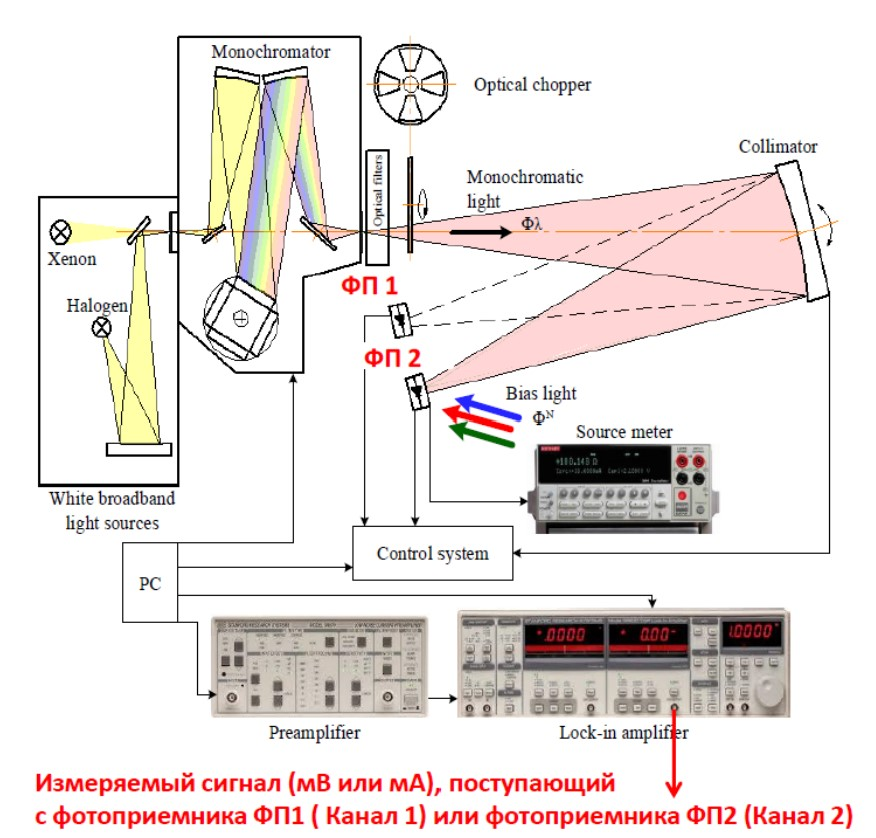
\includegraphics{../image/task.jpg}
		\caption{Схема установки для исследования фотоэлектрических характеристик.}
		\label{w_pert}
	\end{figure}
	
	Калибровка датчика ФП1 производится по эталону ФП2. Зависимость между квантовыми эффективностями датчиков предполагается одинаковой для каждой пары измерений
	\begin{equation}
		QE_{ФП2} = \frac{I_{ФП2}}{I_{ФП1}}*QE_{ФП1} 
		\label{T}
	\end{equation}
	QE - квантове эффективности эталонного и исследуемого датчиков, I - измеренные токи.
	
	\textbf{Исходные данные.}
	Имеется 2 выборки данных с интервальной неопределенностью. Одна из них относится к эталонному датчику ФП2, другая - к исследуемому датчику ФП1.
	
	\textbf{Задача.}
	Треубется определить коэффициент калибровки
	\begin{equation}
		R_{21} = \frac{I_{2}}{I_{1}}
		\label{T}
	\end{equation}
	при помощи линейной регрессии на множестве интервальных данных и коэффициента Жаккара.
	\newpage
	\section{Теория}
	\subsection{Представление данных}
	
	В первую очередь прдставим данные таким образом, чтобы применить понятия статистики данных с интервальной неопределенностью.
	
	Один из распространённых способов получения интервальных результатов в первичных измерениях - это "обинтерваливание" точечных значений, когда к точечному базовому зачению $x_0$, которое считывается по показаниям измерительного прибора, прибавляется
	\textit{интервал погрешности} $\epsilon$:
	
	\begin{equation}
		\textbf{x}=\overset{.}{x}+ \mathbf{\epsilon}
	\end{equation}
	
	Интервал погрешности зададим как
	\begin{equation*}
		\mathbf{\epsilon}=[-\epsilon;\epsilon]
	\end{equation*}
	
	В конкретных измерениях примем $\epsilon$ = $10^{-4}$ мВ.
	
	Согласно терминологии интервального анализа, рассматриваемая выборка - это вектор интервалов, или интервальный вектор $x=(x_1, x_2, ..., x_n)$.
	
	\subsection{Линейная регрессия}
	\subsubsection{Описание модели}
	Линейная регрессия - регрессионная модель зависимости одной переменной от другой с линейной функцией зависимости:
	\begin{equation*}
		y_i = X_ib_i + \epsilon_i
	\end{equation*}
	где X - заданные значения, y - параметры отклика, $\epsilon$ - случайная ошибка модели.
	В случае, если у нас $y_i$ зависит от одного параметра $x_i$, то модель выглядит следующим образом:
	\begin{equation}
		y_i = b_0 + b_1*x_i + \epsilon_i
	\end{equation}
	В данной можели мы пренебрегаем прогрешностью и считаем, что она получается при измерении $y_i$.
	
	\subsubsection{Метод наименьших модулей}
	Для наиболее точного приближения входных с фотоприемников данных $y_i$ линейной регрессией $f(x_i)$ используется метод наименьших модулей. Этот метот основывается на минимизации нормы разности последовательности:
	\begin{equation}
		\| f(x_i) - y_i\|_{l^1} \rightarrow min
	\end{equation}
	В данном случае ставится задача линейного программирования, решение которой дает нам коэффициенты $b_0$ и $b_1$, а также вектор множителей коррекции данных w.
	По итогу получается следующая задача линейного программирования
	\begin{equation}
		\sum_{i=1}^n |w_i| \rightarrow min
	\end{equation}
	\begin{equation}
		b_0 + b_1*x_i - w_i * \epsilon \leq y_i, i = 1..n
	\end{equation}
	\begin{equation}
		b_0 + b_1*x_i + w_i * \epsilon \leq y_i, i = 1..n
	\end{equation}
	\begin{equation}
		1 \leq w_i , i = 1..n
	\end{equation}
	
	\subsection{Предварительная обработка данных}
	Для оценки постоянной, как можно будет увидет далее,  необходима предварительная обработка данных. Займемся линейной моделью дейфа.
	
	\begin{equation}
		Lin(n) = A + B * n, n = 1, 2, ... N
	\end{equation}
	
	Поставив и решив задачу линейного программирования, найдем коэффициенты A, B и вектор w множителей коррекции данных для каждого из фотоприемников ФП1 и ФП2: для данных с первого фотоприемника А = 4.74835, В = $9.17308*10^{-6}$, а для данных со второго - А = 5.18171, В = $1.10476*10^{-5}$. В последствии множитель коррекции данных необходимо применить к погрешностям выборки, чтобы получить данные, которые согласовывались с линейной моделью дрейфа:
	\begin{equation}
		I^f(n) = \overset{.}{x}(n) + \epsilon * w(n), n = 1, 2, ... N
	\end{equation}
	
	По итоге необходимо построить "спрямленные" данные выборки: получить их можно путем вычитания из исходных данных линейную компоненту:
	\begin{equation}
		I^c(n) = I^f(n) - B * n, n = 1, 2, ... N
	\end{equation}
	
	\subsection{Коэффициент Жаккара}
	Коэффициент Жаккара - мера сходства множеств. В интервальных данных рассматривается некоторая модификация этого коэффициента: в качестве меры множества (в данном случае интервала) рассматривается его длина, а в качестве пересечения и оъединения - взятие минимума и максимума по включению двух величин в интервальной арифметике Каухера соответственно. Можно заметить, что в силу возможности минимума по включению быть неправильным инервалом, коэффициент Жаккара может достишать значения только в интервале [-1; 1].
	\begin{equation}
		JK(x) = \frac{wid(\wedge x_i)}{wid(\vee x_i)}
	\end{equation}
	
	\subsection{Процедура оптимизации}
	Чтоб найти оптимальный параметр калиброфки $R_21$ необходимо поставить и решить задачу максимизации коэффициента Жаккара, зависящего от парамертра калибровки:
	\begin{equation}
		JK(I_1^c(n) * R \cup I_2^c(n)) =  \rightarrow max
	\end{equation}
	где $I_1^c$ и $I_2^c$ - полученные спрямленные выборки, а R - параметр калибровки. Найденный таким образом R и будет искомым оптимальным $R_{21}$ в силу наибольшего совпадения, оцененного коэффицентом Жаккара.
	\section{Реализация}
	\subsection{Описание}
	Данная лабораторная работа была выполнена с использованием языка
	программирования Python 3.10 в среде разработки PyCharm с
	использованием следующих библиотек:
	\begin{itemize}
		\item math - использование математических функций
		\item matplotlib версии 3.7.1 - построение графиков
		\item numpy версии 1.24.2 - использование многомерных массивов
		\item prettytable версии 3.6.0 - вывод таблиц в консоли 
		\item scipy версии 1.10.1 - статические распределения и функции
		\item seaborn версии 0.12.2 - посроение графиков, визуализация
		\item statsmodels - дополнение к scipy, использование статистических вычислений, включая описательную статистику, оценку и вывод статистических моделей
	\end{itemize}
	Отчёт подготовлен с помощью языка LaTEX в редакторе TexStudio.
		\subsection{Ссылка на репозиторий}
		\url{https://github.com/IMZolin/Math-statistics-labs} \ - GitHub репозиторий
	
	\section{Результаты}
	\begin{figure}[H]
		\begin{tabular}{ccc}
			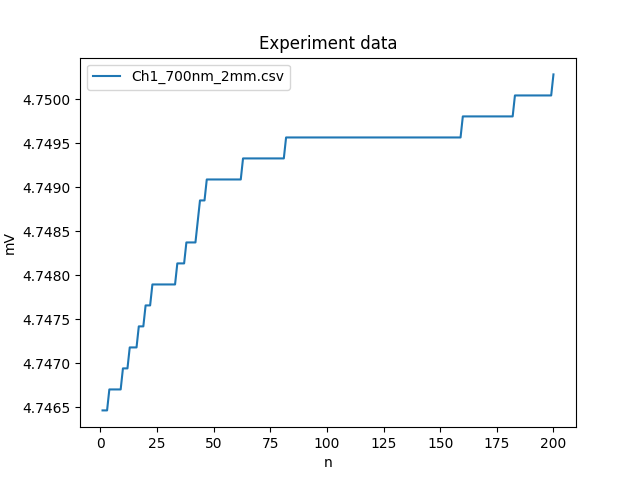
\includegraphics[scale=0.5]{../image/input_PR1.png}
			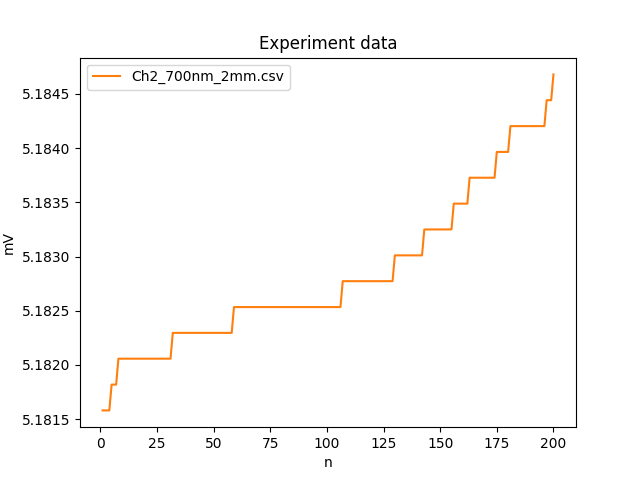
\includegraphics[scale=0.5]{../image/input_PR2.png}
		\end{tabular}
		\caption{Исходные данные из экспериментов} 
	\end{figure}
	
	\begin{figure}[H]
		\begin{tabular}{ccc}
			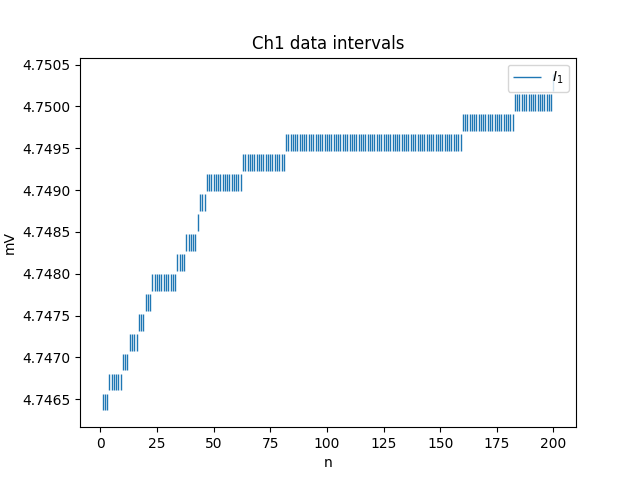
\includegraphics[scale=0.5]{../image/intervals_PR1.png}
			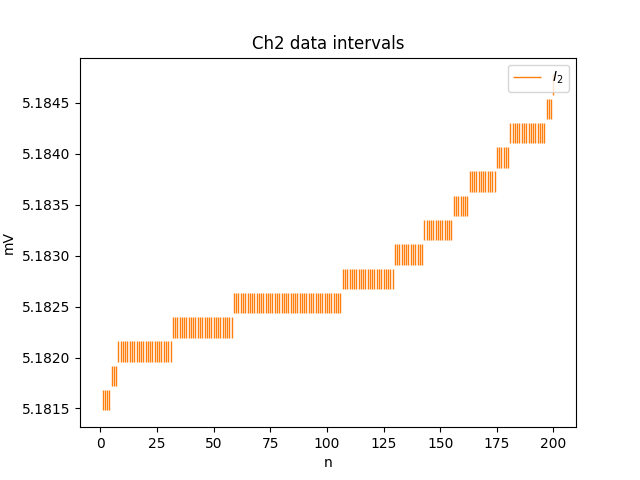
\includegraphics[scale=0.5]{../image/intervals_PR2.png}
		\end{tabular}
		\caption{Интервальное представление исходных данных} 
	\end{figure}
	
	\begin{figure}[H]
		\begin{tabular}{ccc}
			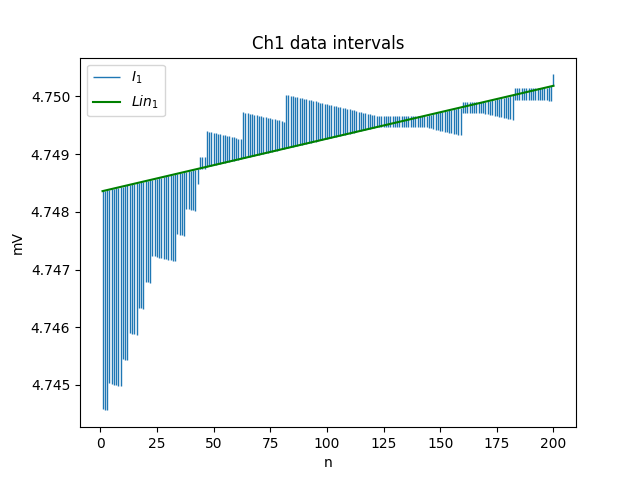
\includegraphics[scale=0.5]{../image/lr_PR1.png}
			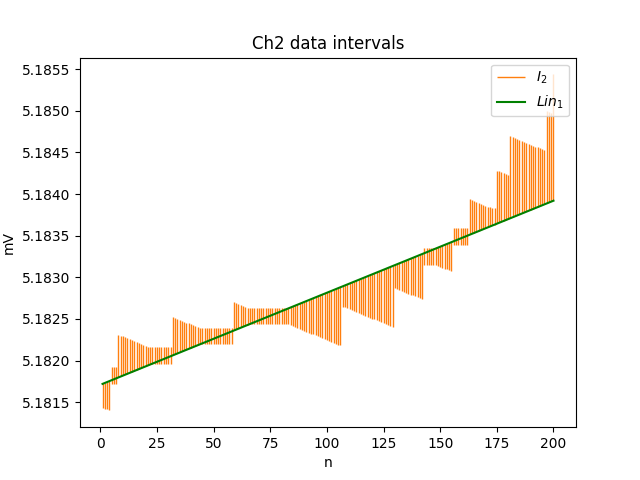
\includegraphics[scale=0.5]{../image/lr_PR2.png}
		\end{tabular}
		\caption{Линейная модель дрейфа данных} 
	\end{figure}
	
	\begin{figure}[H]
		\begin{tabular}{ccc}
			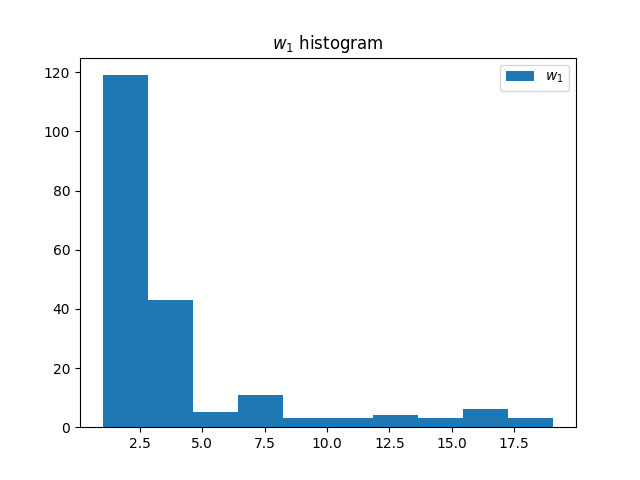
\includegraphics[scale=0.5]{../image/whyst_PR1.png}
			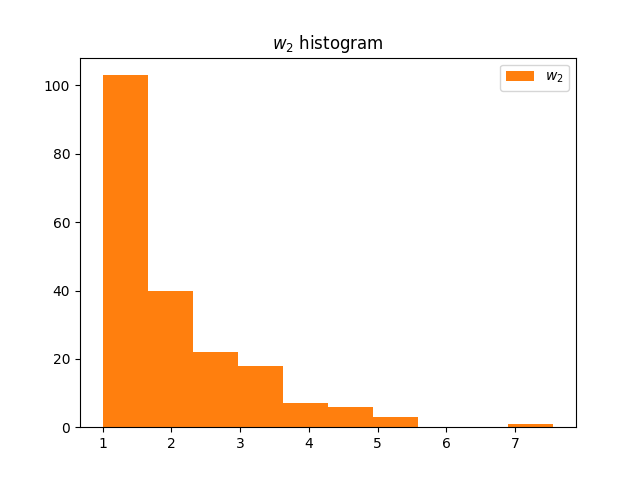
\includegraphics[scale=0.5]{../image/whyst_PR2.png}
		\end{tabular}
		\caption{Гистограммы значений множителей коррекции w} 
	\end{figure}
	
	\begin{figure}[H]
		\begin{tabular}{ccc}
			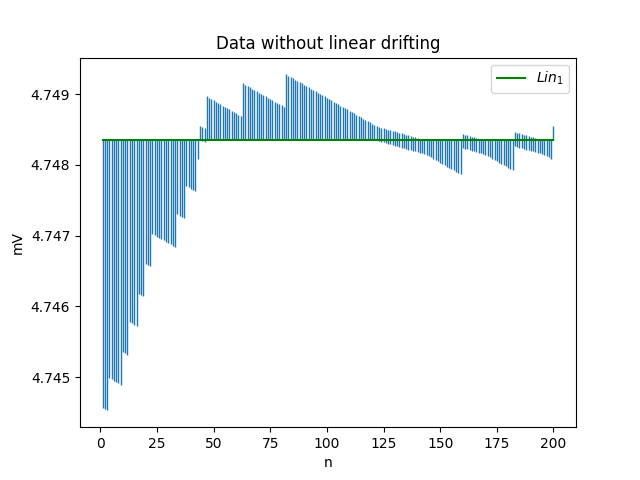
\includegraphics[scale=0.5]{../image/fixed_PR1.png}
			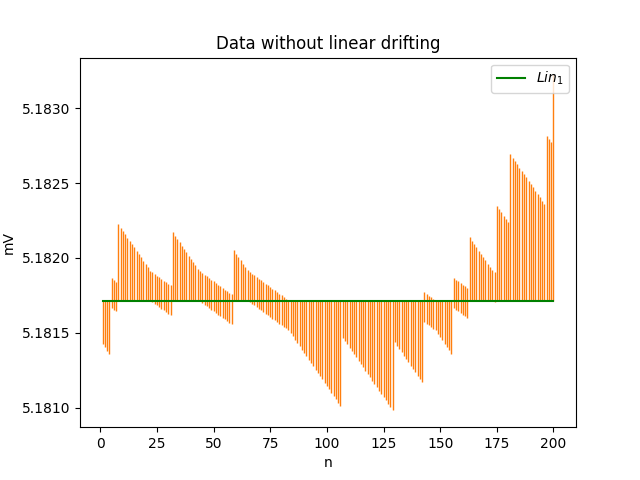
\includegraphics[scale=0.5]{../image/fixed_PR2.png}
		\end{tabular}
		\caption{Скорректированные модели данных} 
	\end{figure}
	
	\begin{figure}[H]
		\begin{tabular}{ccc}
			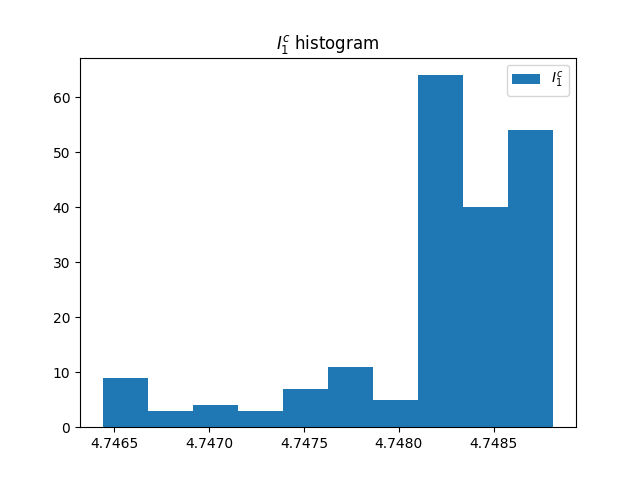
\includegraphics[scale=0.5]{../image/fhyst_PR1.png}
			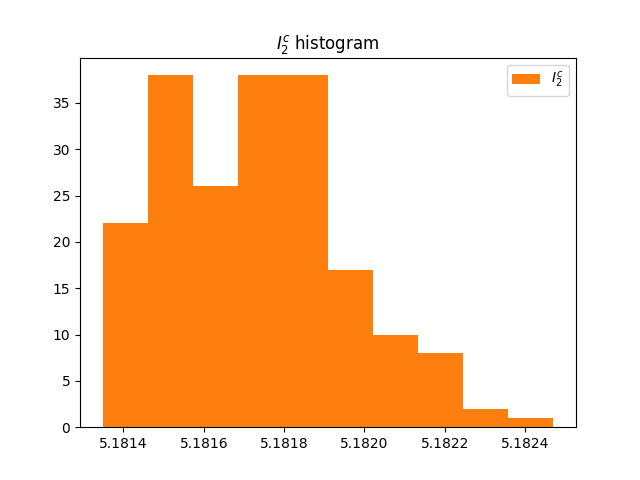
\includegraphics[scale=0.5]{../image/fhyst_PR2.png}
		\end{tabular}
		\caption{Гистограммы скорректированных данных} 
	\end{figure}
	
	\begin{figure}[H]
		\begin{tabular}{ccc}
			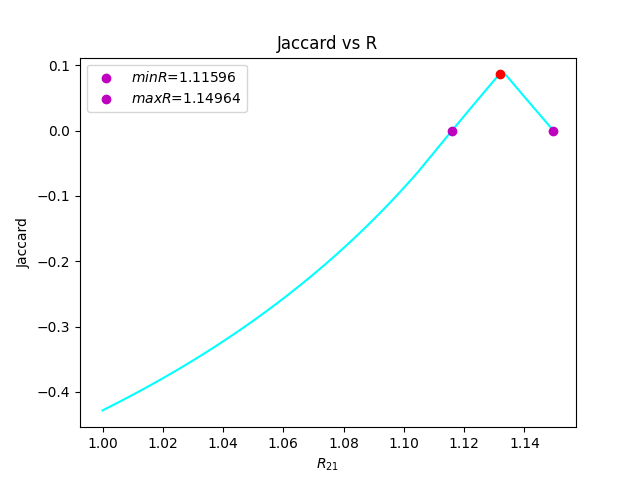
\includegraphics[scale=0.5]{../image/jakkar.png}
			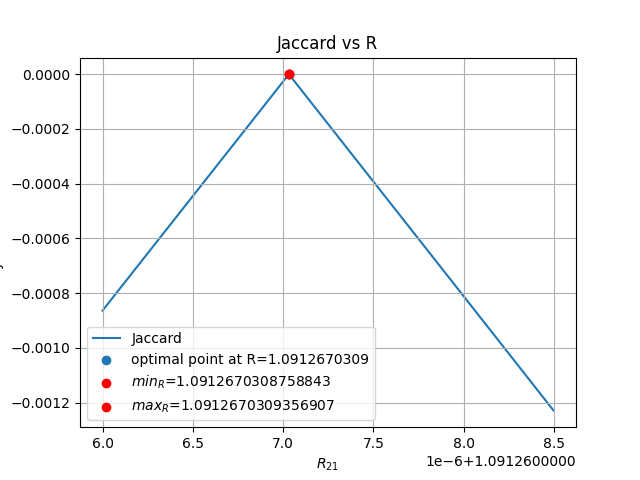
\includegraphics[scale=0.5]{../image/jakkar(smol).png}
		\end{tabular}
		\caption{Значение коэффициента Жаккара от калибровочного множителя от $R_{21}$} 
	\end{figure}
	
	\begin{figure}[H]
		\begin{center}
			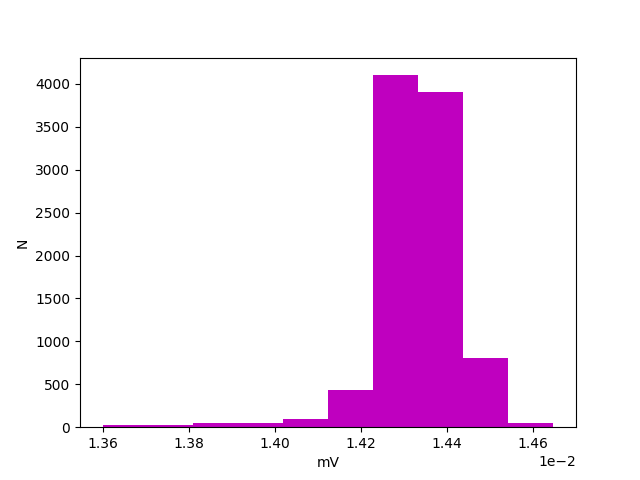
\includegraphics[scale=0.5]{../image/jakkar_combined_hist.png}
		\end{center}
		\caption{Гистограмма объединнённых данных при оптимальном значении $R_{21}$} 
	\end{figure}
	
	\section{Обсуждение}
	\textbf{Множители коррекции w.}
	На гистограммах значений множителей коррекции (Рис.5), видно, что половина (для эталлоного фотопередатчика даже больше) не требует коррекции. Это означает, что линейная модель дрейфа данных является разумным приближением.
	
	
	
	\textbf{Коэффициент Жаккара}
	На рис.8 видно, что оптимальным множителем $R_{21}$ является число, равное 1.0912670309. Однако видно, что коэффициент Жаккара при оптимальном значении едва-едва превышает 0, а интервал, при котором JK $\geq$ 0, соизмерим с точкой (длина интервала оценивается $10^{-9} - 10^{-10} $). Это показывает на то, что исходные данные имеют ряд неточностей, которые сложно устранить. Это же можно было и заметить на Рис.3, иллюстрирующий входные данные. Однако, как будет далее видно, подобранный коэффициент $R_{21}$ приблизит данные первого фотоприемника к данным второго фотоприемника.
	
	
	
	\textbf{Гистограмма объединённых данных при оптимальном значении R.}
	Сравнивая гистограмму объединённых данных при оптимальном значении $R_{21}$ (Рис. 9) с гистограммами скорректированных данных (Рис. 7), видно, что гистограмма объединённых данных повторяет форму гистограммы входных данных с ФП1, однако пик гистограммы смещен в сторону значения пика на гистограмме ФП2.
	

	\newpage
	\addcontentsline{toc}{section}{Литература}
	
	\begin{thebibliography}{4}
		\bibitem{s:hist}
		Histogram. URL: \url{https://en.wikipedia.org/wiki/Histogram}
		\bibitem{b:probSectMath}
		Вероятностные разделы математики. Учебник для бакалавров технических направлений.//Под ред. Максимова Ю.Д. --- Спб.: «Иван Федоров», 2001. --- 592 c., илл.
		\bibitem{s:boxplot}
		Box plot. URL: \url{https://en.wikipedia.org/wiki/Box_plot}
		\bibitem{a:nonParamRegr}
		Анатольев, Станислав (2009) «Непараметрическая регрессия», Квантиль, №7, стр. 37-52.
		\bibitem{a:nonParamRegr} М.З.Шварц. Данные технологических испытаний оборудования для калибровки фотоприемников солнечного излучения. 2022.
	\end{thebibliography}

\end{document}